\chapter{Low temperature environments}
\section{Introduction}
\begin{itemize}
    \item Low temperature: \SI{-273}{\degree C}, \SI{-150}{\degree C}
    \item Mechanical challenges - rapid heating / increasing gas pressure
          \begin{itemize}
              \item Failure / fatigue
          \end{itemize}
    \item Most low temperature - rise at atmospheric pressure
          \begin{itemize}
              \item Small volumes
          \end{itemize}
    \item Through design - challenge becomes managing the thermal component not the mechanical
    \item Health \& Safety - dense / cold gas moves quickly and can suffocate people
\end{itemize}
\begin{table}[H]
    \centering
    \begin{tabular}{@{}ll@{}}
        \toprule
        \textbf{Gas} & \textbf{Freezing temperature}      \\
        \midrule
        \ce{CO2}     & \SI{-78.5}{\degree C} (sublimates) \\
        Nitrogen     & \SI{-196}{\degree C}               \\
        LNG          & \SI{-161.5}{\degree C}             \\
        \bottomrule
    \end{tabular}
    \caption{Freezing temperatures of various gases.}
\end{table}
The energy density of LNG is comparable to propane and ethanol but is only 60 percent that of diesel and 70 percent that of gasoline.
\begin{figure}[H]
    \centering
    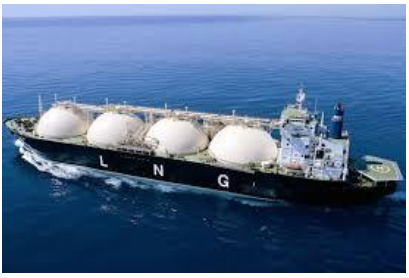
\includegraphics[width = 0.5 \textwidth]{img/figure56.png}
    \caption{LNG carrier.}
\end{figure}
An LNG carrier is a tank ship designed for transporting liquefied natural gas. At the end of 2016, the global LNG shipping fleet consisted of 439 vessels. Majority of ships have a capacity of \SI{120000}{}-\SI{140000}{\meter\cubed}.
\begin{table}[H]
    \centering
    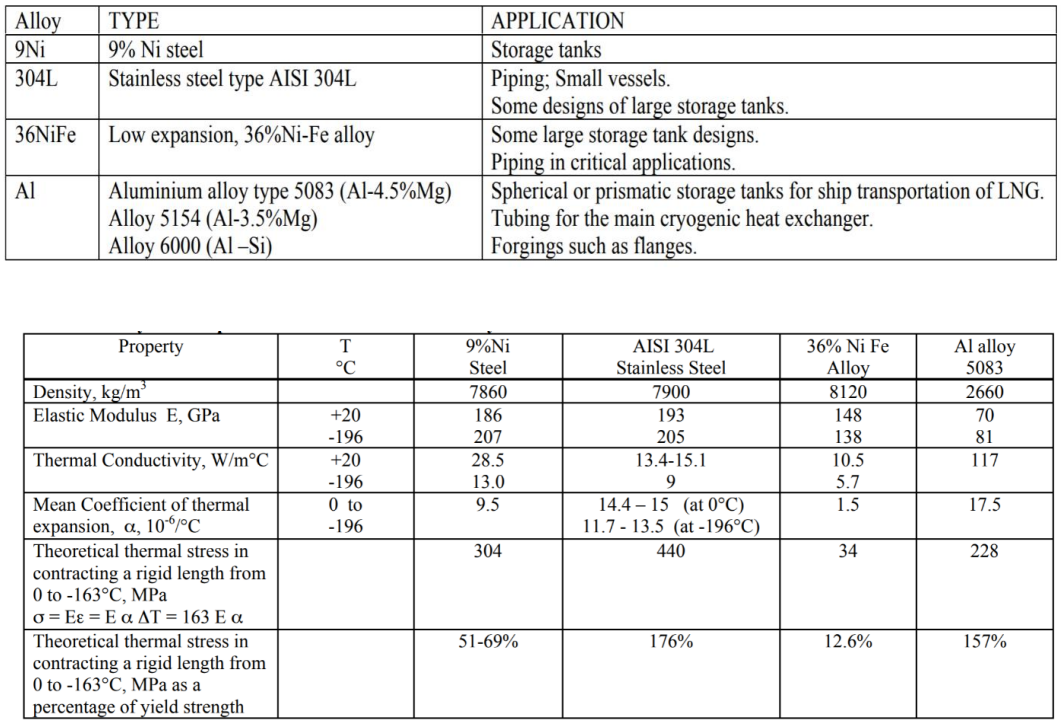
\includegraphics[width = \textwidth]{img/figure57.png}
    \caption{Tables to show material properties of storage tanks.}
\end{table}
\begin{table}[H]
    \centering
    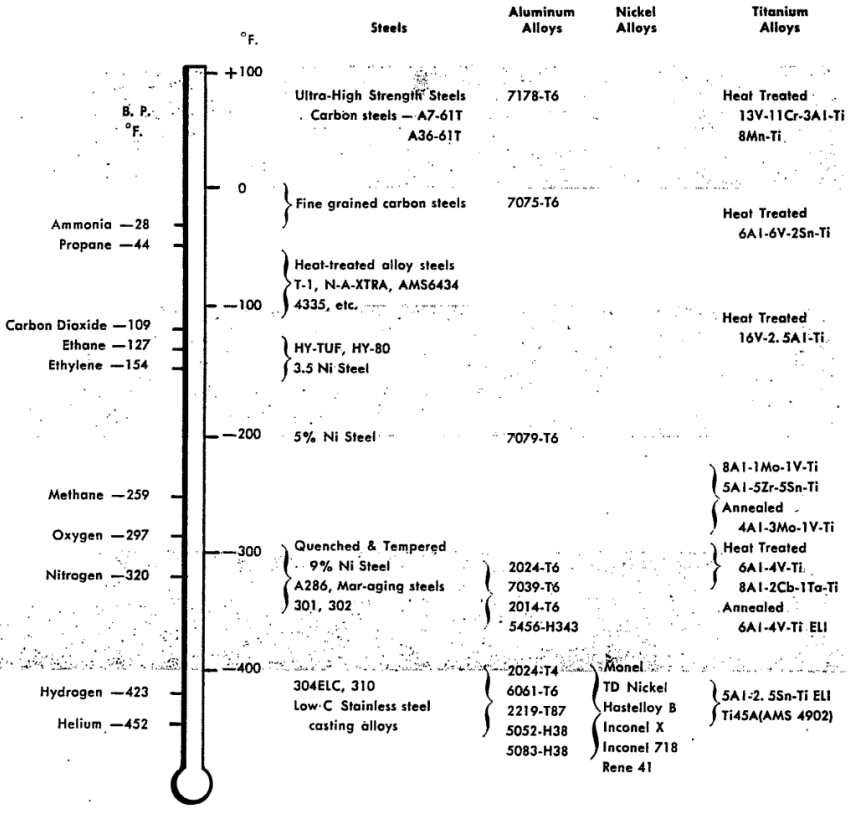
\includegraphics[width = \textwidth]{img/figure58.png}
    \caption{Table to show materials used to store different low temperature materials.}
\end{table}
\section{Engineering applications}
\subsection{LNG - liquefied natural gas}
Methane, \ce{CH4} (with some ethane). 1/6000$^{\textrm{th}}$ the volume of natural gas in the gaseous state (at standard condition for temperature and pressure). It is odourless, colourless, non-toxic and non-corrosive. Hazards include flammability after vaporisation into a gaseous state, freezing and asphyxia. The liquefaction process involves removal of certain components, such as dust, acid gases, helium, water and heavy hydrocarbons, which could cause difficulty downstream. The natural gas is then condensed into a liquid at close to atmospheric pressure by cooling it to approximately \SI{-162}{\degree C}. Maximum transport pressure is set at around \SI{25}{\kilo\pascal}.
\subsection{Cryogenic transport}
Transfer lines are a form of cryostat. Used to transport cryogenic fluids between cryogenic devices. Simplest form is a vacuum jacketed pipe connecting two flasks. Heat is absorbed by the liquid (nitrogen) and as the pipe gets longer, more heating occurs and more vapour generated (which is lost). Higher pressure differential, more heating occurs. The most important design elements are:
\begin{itemize}
    \item Geometry
    \item Mass flow rate
    \item Temperature and pressure change
    \item Cryogenic fluid
    \item Mechanical properties of the materials
\end{itemize}
\section{Thermal bowing}
\begin{figure}[H]
    \centering
    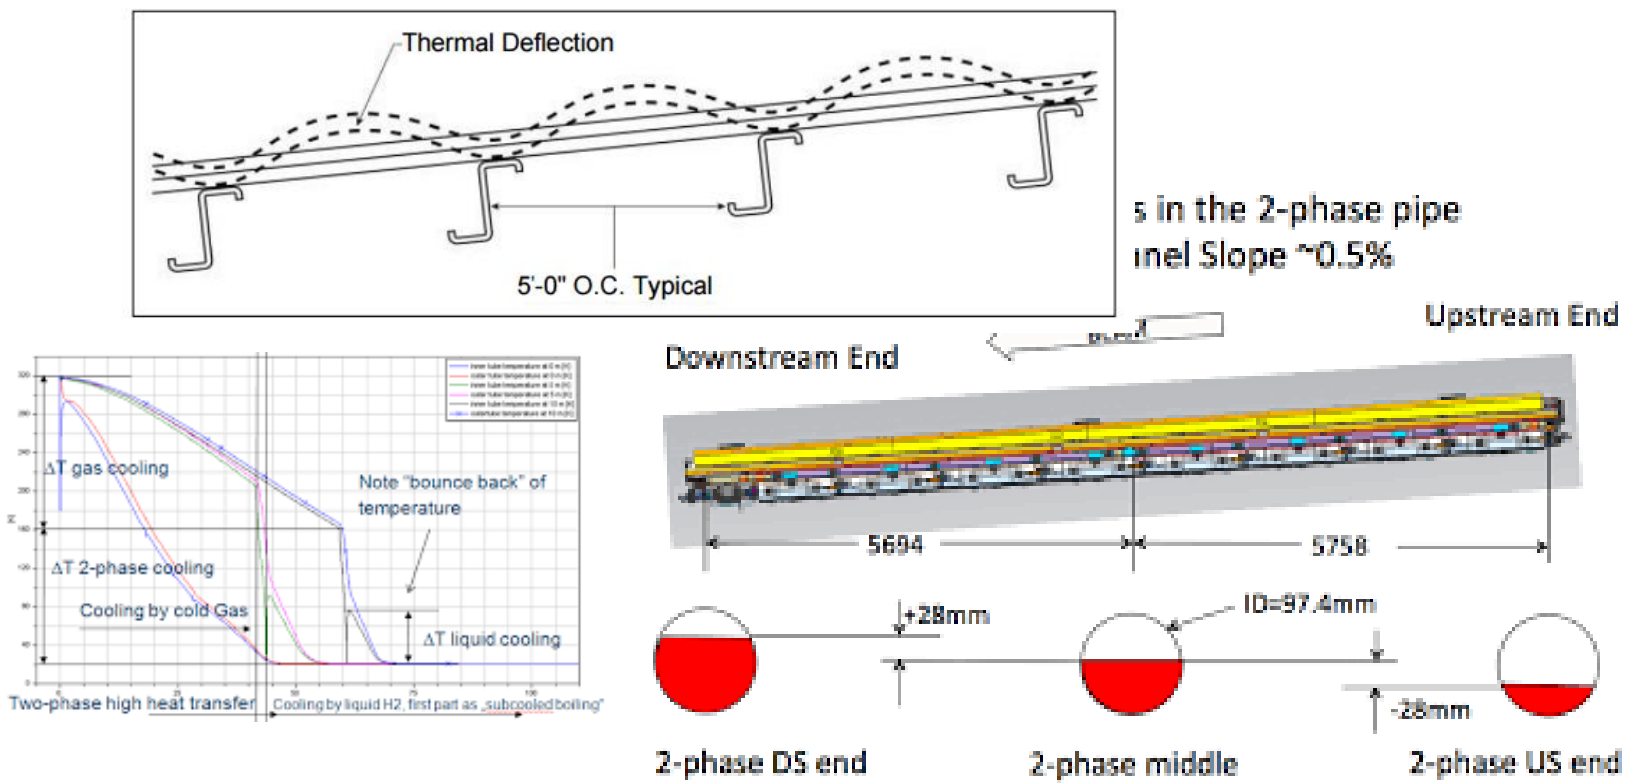
\includegraphics[width = \textwidth]{img/figure59.png}
    \caption{Thermal bowing.}
\end{figure}
\subsubsection{Laterial variation of temperature}
Thermal bowing occurs due to two processes:
\begin{enumerate}
    \item Restrained thermal expansion
    \item Temperature gradient across pipe
\end{enumerate}
Assuming no mean temperature increase:
\begin{equation}
    \Delta T = 0
\end{equation}
\begin{figure}[H]
    \centering
    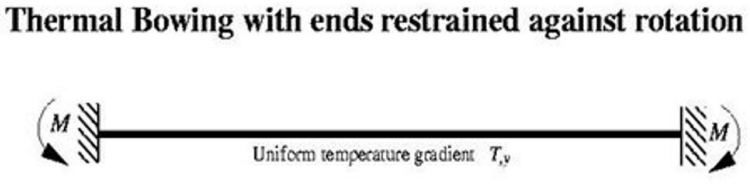
\includegraphics[width = 0.6\textwidth]{img/figure60.png}
    \caption{Fixed end beam subjected to a uniform thermal gradient.}
\end{figure}
Uniform moment over the length:
\begin{equation}
    M = EI \phi = EI\alpha T_{,y}
\end{equation}
\begin{figure}[H]
    \centering
    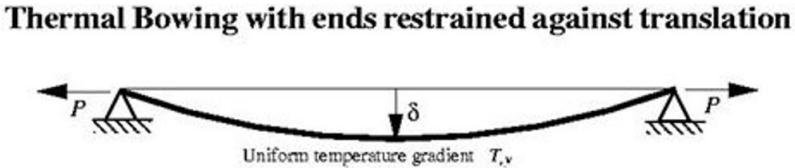
\includegraphics[width = 0.6\textwidth]{img/figure61.png}
    \caption{Laterally restrained beam subjected to a uniform thermal gradient.}
\end{figure}
A tensile force $P$ will be generated causing a tensile $P-\delta$ moment $Py$ over the length of the beam,
\begin{equation}
    \frac{\dif^2 y}{\dif x^2} = \phi + \frac{Py}{EI}
\end{equation}
or
\begin{equation}
    \frac{\dif^2 y}{\dif x^2} - k^2 y = \phi
\end{equation}
where,
\begin{equation}
    K = \sqrt{\frac{P}{EI}}
\end{equation}
The solution of this equation is,
\begin{equation}
    y\left(x\right) = -\frac{\phi}{k^2}\left(\frac{\cosh\left(kl\right) - 1}{\sinh\left(kl\right)}\sinh\left(kx\right)\cosh\left(kx\right)+1\right)
\end{equation}
\subsubsection{Derivation}
The derivation starts with the point that the displacement is:
\begin{equation}
    u = f\left(x\right) + yf_1\left(x\right) + zf_2\left(x\right)
\end{equation}
The longitudinal strain is
\begin{equation}
    \epsilon_{xx} = \frac{\partial u}{\partial x} = f'\left(x\right) + yf_1'\left(x\right) + zf_2'\left(x\right)
\end{equation}
The stress field is
\begin{equation}
    \sigma_{xx} = E \left(\epsilon_{xx} - \alpha T\right)
\end{equation}
The equilibrium constraints are
\begin{align}
    \int \sigma \dif A   & = 0 \\
    \int \sigma y \dif A & = 0 \\
    \int \sigma z \dif A & = 0
\end{align}
The geometrical constraint is
\begin{equation}
    \int y \dif A = \int z \dif A = 0
\end{equation}
Cross-pipe variation of temperature:
\begin{equation}
    \sigma_{xx} = -\alpha E\left(T - \bar{T}\right) + \frac{I_yM_{Tz}-I_{yx}M_{Ty}}{I_yI_z-I^2_{yz}}y + \frac{I_yM_{Tz}-I_{yx}M_{Ty}}{I_yI_z-I^2_{yz}}z
\end{equation}
where
\begin{align}
    I_z    & = \int y^2 \dif A        \\
    I_y    & = \int z^2 \dif A        \\
    I_{yz} & = \int yz \dif A         \\
    M_{Ty} & = \int \alpha ETz \dif A \\
    M_{Tz} & = \int \alpha ETy \dif A
\end{align}
For a pipe
\begin{equation}
    \sigma_{xx} = -\alpha E \left(T - \bar{T}\right) + \frac{M_{Tz}}{I_y}y
\end{equation}
For the lateral displacement
\begin{gather}
    \frac{\dif^2 v}{\dif x^2} = - \frac{M_{Tz}}{EI_z}\\
    \frac{\dif}{\dif x^2}\left(EI_z\frac{\dif^2 v}{\dif x^2}\right) + \frac{\dif^2 M_{Tz}}{\dif x^2} = F
\end{gather}
\begin{figure}[H]
    \centering
    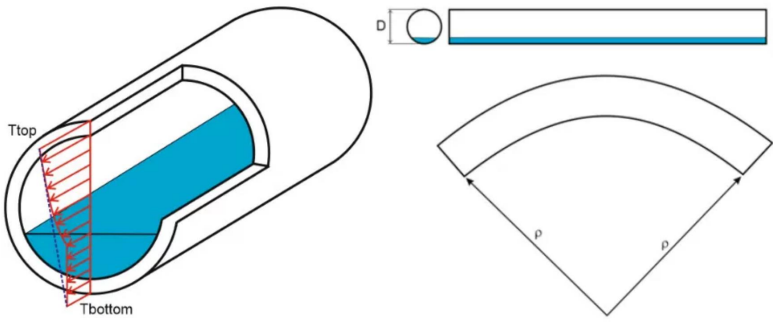
\includegraphics[width = 0.6\textwidth]{img/figure62.png}
    \caption{Cross-section of pipe.}
\end{figure}
\section{Phase change transition}
NG Rapid Phase Transitions (RPT). Rapid changes in phase due to temperature leads to enormous fluid impulse. This causes problems with the piping network. Rapid phase changes leads to a fluid impulse and often regarded as a water hammer. This phenomenon is well known in the context of steam (from the 19$^{\textrm{th}}$ century) - leading it to be called the steam hammer.

In a steam system, a water hammer most often occurs when some of the steam condenses into water in a horizontal section of the piping. The rest of the steam picks up the water, forming a ``slug'', and hurls this at high velocity into a pipe fitting, creating a loud hammering noise and greatly stressing the pipe. This condition is usually caused by a poor condensate drainage strategy: having more condensate in the pipe makes the slug easier to form. Vacuum caused by condensation from the thermal shock can also cause a steam hammer. Steam hammers can be avoided by using sloped pipes and installing steam traps. Where air-filled traps are used, these eventually become depleted of their trapped air over a long period through absorption into the water. This can be  cured by shutting off the supply, opening taps at the highest and lowest locations to drain the system (thereby restoring air to the lowest traps), and then closing the taps and re-opening the supply. 
\section{LNG transport}
The various stages need to be analysed. The first is the transport in the pipe. The second is the filling the space. The third is the environmental challenges - phase change water hammer. 
\subsubsection{Moss tanks}
Named after the company that designed them, the Norwegian company Moss Maritime, the spherical IMO type B LNG tanks are spherical in shape. Most Moss type vessels have four or five tanks. 

The outside of the tank has a thick layer of foam insulation that is either fitted in panels or in more modern designs, wound round tank. Over this insulation is a thin layer of ``tinfoil'' which allows the insulation to be kept dry with a nitrogen atmosphere. This atmosphere is constantly checked for any methane that would indicate a leak of the tank. Also the outside of tank is checked at three month intervals for any cold spots that would indicate breakdown in the insulation.

The tank is supported around its circumference by the equatorial ring which is supported by a large circular skirt which takes the weight of the tank down to the ships structure. This skirt allows the tank to expand and contract during cool-down and warm-up operations. During cool-down or warm-up, the tank can expand or contract about \SI{60}{\centi\meter}. Because of this expansion and contraction all piping into the tank comes in the top and is connected to the ships lines via flexible bellows. 

Inside ach tank there is a set of spray heads. These heads are mounted around the equatorial ring and are used to spray liquid LNG onto the tank walls to reduce the temperature. 

Tanks normally have a working pressure of up to \SI{22}{\kilo\pascal}, but this can be raised for an emergency discharge. If both main pumps fail then to remove cargo, the tank's safety valves are adjusted to lift at \SI{1}{bar}. Then the filling line which goes to the bottom of the tank is opened along with the filling lines of the other tanks on board. THe pressure is then raised in the tank with the defective pumps which pushes the cargo into the other tanks where it can be pumped out.
\subsubsection{TGZ Mark III}
Designed by Technigaz, these tanks are of the membrane type. The membrane consists of stainless steel with `waffles' to absorb the thermal contraction when the tank is cooled down. The primary barrier, made of corrugated stainless steel of about \SI{1.2}{\milli\meter} thickness is the one in direct contact with the cargo liquid (or vapour in the empty tank condition). This is followed by a primary insulation which in turn is covered by a secondary barrier made of a material called `triplex' which is basically a metal foil sandwiched between glasswool sheets and compressed together. This is again covered by a secondary insulation which in turn is supported by the ship's hull structure from the outside. 

From the inside of the tank outwards, the layers are:
\begin{enumerate}
    \item LNG
    \item Primary barrier of \SI{1.2}{\milli\meter} thick corrugated / waffled 304L stainless steel
    \item Primary insulation (also called the interbarrier space)
    \item Secondary barrier within the triplex membrane
    \item Secondary insulation (also called the insulation space)
    \item Ship's hull structure
\end{enumerate}
\begin{figure}[H]
    \centering
    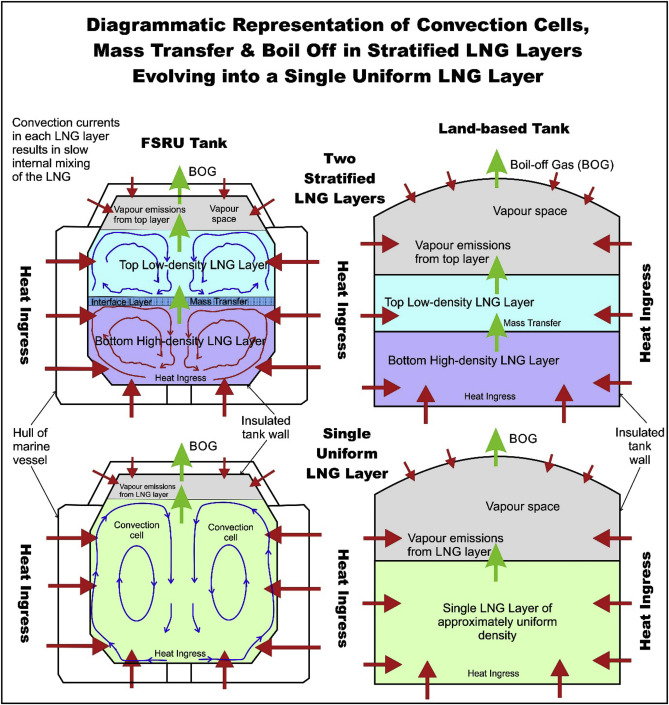
\includegraphics[width = 0.8\textwidth]{img/figure63.jpg}
    \caption{LNG rollover.}
\end{figure}
LNG ``rollover'' refers to the rapid release of LNG vapours from a storage tank caused by stratification. The potential for rollover arises when two separate layers of different densities (due to different LNG compositions) exist in a tank. In the top layer, liquid warms up due to heat leakage into the tank, rises up to the surface, where it evaporates. Thus light gases are preferentially evaporated and the liquid in the upper layer becomes denser. This phenomenon is called ``weathering''. In the bottom layer, the warmed liquid rises to the interface by free convection but does not evaporate due to the hydrostatic head exerted by the top layer. Thus the lower layer becomes warmer and less dense. As the density of two layers approach each other, the two layers mix rapidly, and the lower layer which has been superheated gives off large amount of vapour as it rises to the surface of the tank.
\subsubsection{Reduction of explosion risk}
Tanks are filled via a series of stages
\begin{enumerate}
    \item Flush tank with \ce{CO2} from the exhaust. This is because LNG and air mixture is flammable
    \item Fill with LNG at ambient temperature and pressure
    \item Vessel goes into port to ``gas-up'' and ``cool-down'', as one still cannot load directly into the tank: the \ce{CO2} will freeze and damage the pumps and the cold shock could damage the tank's pump column
    \item LNG is brought onto the vessel and taken along the spray line to the main vaporiser, which boils off the liquid into gas. This is then warmed up to roughly \SI{20}{\degree C} in the gas heaters and then blown into the tanks to displace the ``inert gas''. This continues until all the \ce{CO2} is removed from the tanks. Initially the IG (inert gas) is vented to atmosphere. Once the hydrocarbon content reaches 5\% (lower flammability range of methane) the inert gas is redirected to shore via a pipeline and manifold connection by the HD (high duty) compressors. This shore terminal then burns this vapour to avoid the dangers of having large amounts of hydrocarbons around which may explode
    \item Now the vessel is gassed up and warm. The tanks are still at ambient temperature and are full of methane
    \item The next stage is cool-down. LNG is sprayed into the tanks via spray heads, which vaporises and starts to cool the tank. The excess gas is again blown ashore to be re-liquefied or burned at a flare stack. Once the tanks reach about \SI{-140}{\degree C} the tanks are ready to load bulk
    \item Bulk loading starts and liquid LNG is pumped from the storage tanks ashore into the vessel tanks. Displaced gas is blown ashore by the HD compressors. Loading continues until typically 98.5\% full is reached (to allow for thermal expansion / contraction of cargo)
    \item The vessel can now proceed to the discharge port. During passage, various boil-off management strategies can be used. Boil-off gas can be burned in boilers to provide steam for propulsion, or it can be re-liquefied and returned to the cargo tanks, depending on the design of the vessel
\end{enumerate}
\subsubsection{Above ground full containment LNG tank design}
\begin{figure}[H]
    \centering
    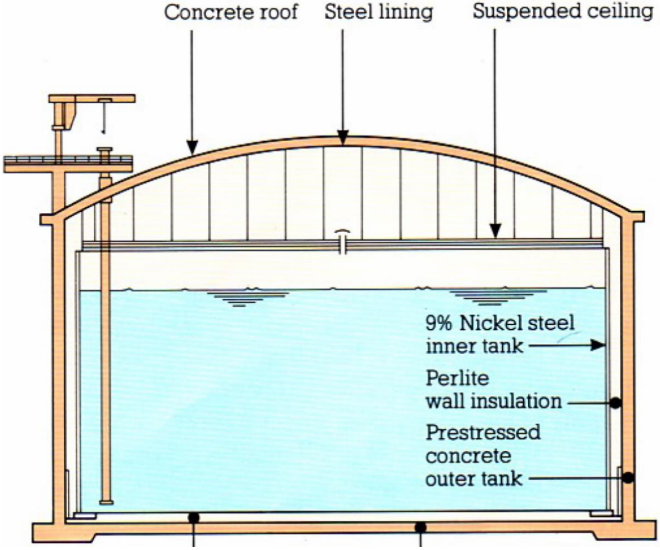
\includegraphics[width = 0.6\textwidth]{img/figure64.png}
    \caption{Above ground full containment LNG tank design.}
\end{figure}
\begin{itemize}
    \item Pre-stressed concrete outer walls constructed by slipforming, sheathed internally with a gas-tight layer of nickel-alloyed steel
    \item Inner tank in nickel-alloyed steel, separated from the outer walls by a layer of perlite - a variety of volcanic obsidian highly suitable for insulation
    \item Extra layer of steel and insulation at the transition between outer wall and tank bottom to protect it against strong local stresses should the inner tank begin to leak
    \item Heating cables under the tanks will ensure that ground remains above \SI{0}{\degree C} in order to prevent frost heaving
\end{itemize}
\subsubsection{Rollover}
Rollover is a phenomenon that can occur when LNG at different density / temperature is filled into a storage tank. LNG composition, density and temperature will change during boil-off gas. If not mixed, a high density liquid will settle below the lower density liquid. During heat leakage and evaporation, the density of the upper level of liquid can become higher than the lower level of liquid and a sudden rollover with mixing of the liquids may occur giving sudden evaporation and pressure build up, which can lead to tank rupture. In 1971, a rollover incident happened at the La Spezia LNG import terminal in Italy and damaged the tank roof. No ignition happened. Receiving terminals now have procedures to mix old and new LNG during filling. LNG tanks have rollover protection systems which include distributed temperature sensors and pump-around mixing systems.
\begin{figure}[H]
    \centering
    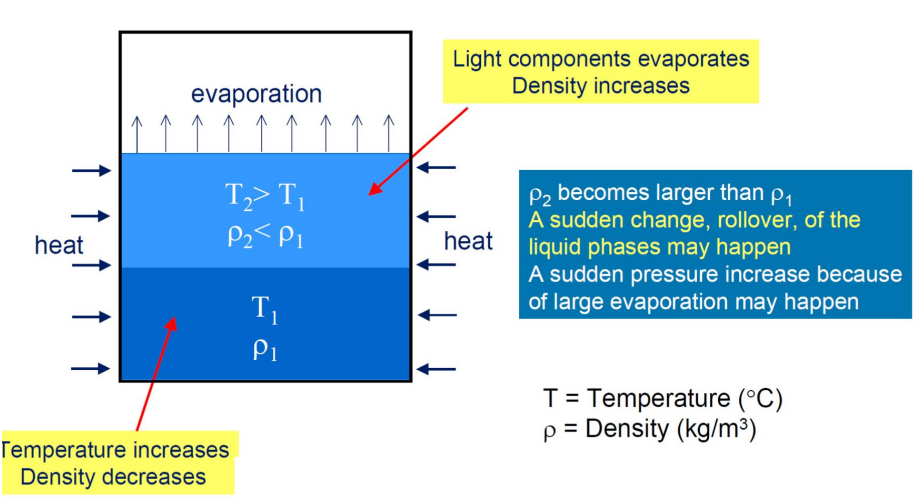
\includegraphics[width = 0.8\textwidth]{img/figure65.png}
    \caption{Mechanics of rollover in LNG tanks.}
\end{figure}
\begin{figure}[H]
    \centering
    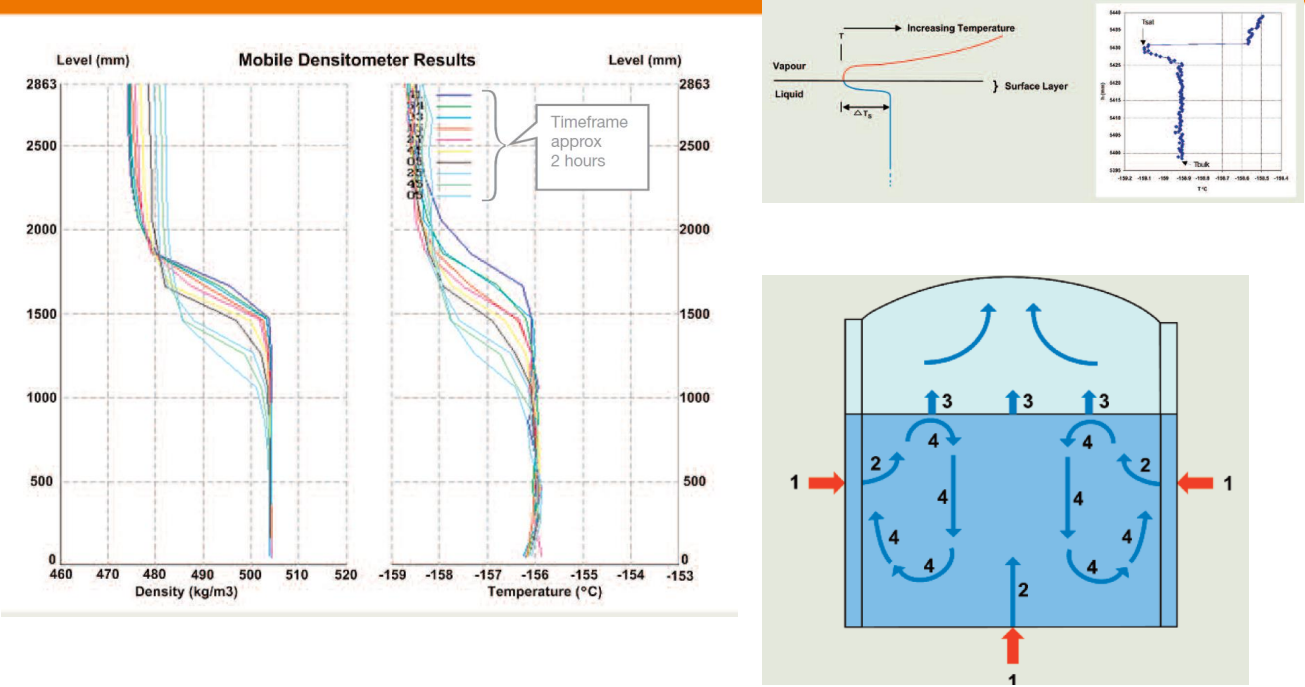
\includegraphics[width = 0.8\textwidth]{img/figure66.png}
    \caption{Measurement of LNG density in tank.}
\end{figure}
\section{Sub 4K refrigeration system}
Cooling using a refrigeration system. Also can use paramagnetic materials. Helium is expensive so everything is recovered. Usually \ce{He} is delivered at \SI{4.5}{\kelvin} \SI{3}{bar}. \SI{2}{\kelvin} helium is produced by a cryogenic device. Issue to do with pressure for a helium transport. 
\subsubsection{Transfer lines}
Cryogenic transfer lines are modular. They usually consist of multichannel components.
\begin{enumerate}
    \item Thermal shield
    \item External envelope
    \item Vacuum barrier
    \item Sliding support
    \item Fixed supports
\end{enumerate}
Both process and external envelope contain internal bellows to account for the shrinkage of pipes.
\begin{figure}[H]
    \centering
    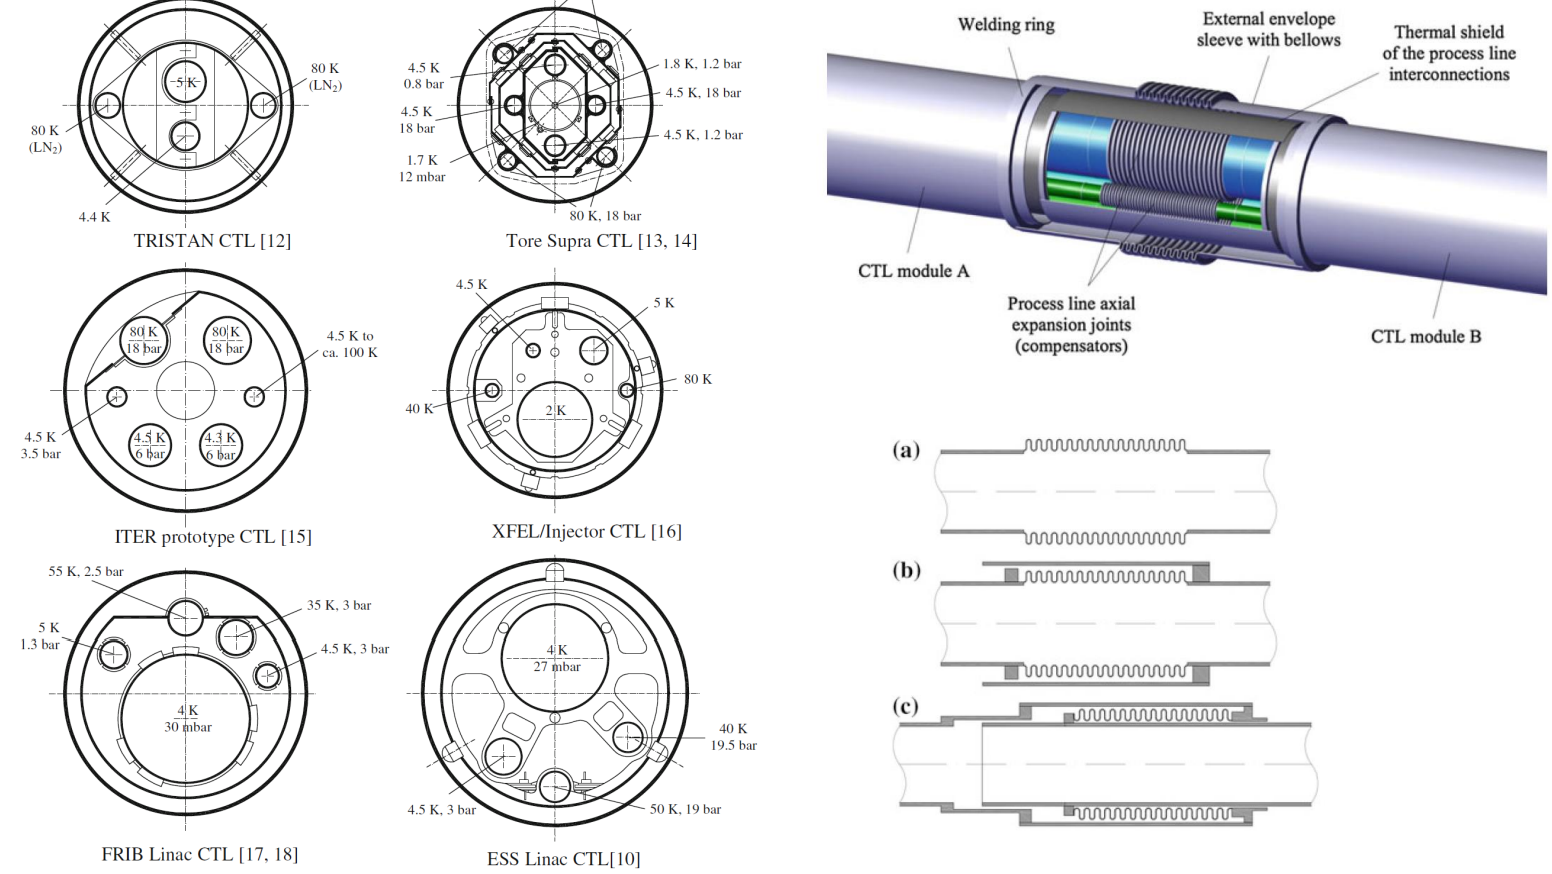
\includegraphics[width = 0.8\textwidth]{img/figure67.png}
    \caption{Cryogenic transfer line cross-section and sliding support mechanism.}
\end{figure}
\begin{figure}[H]
    \centering
    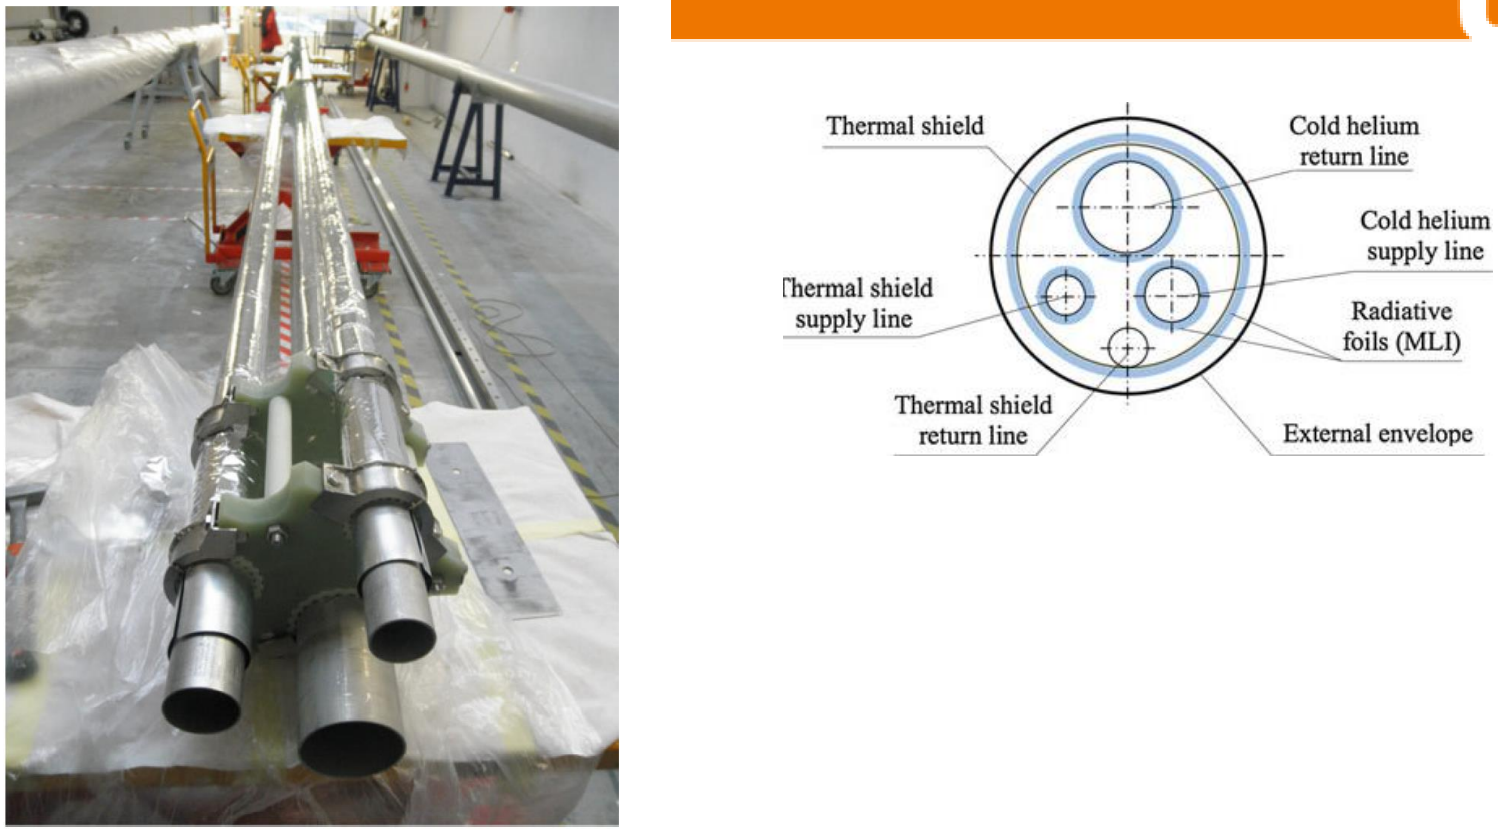
\includegraphics[width = 0.8\textwidth]{img/figure68.png}
    \caption{Cryogenic transfer line components.}
\end{figure}
\begin{table}[H]
    \centering
    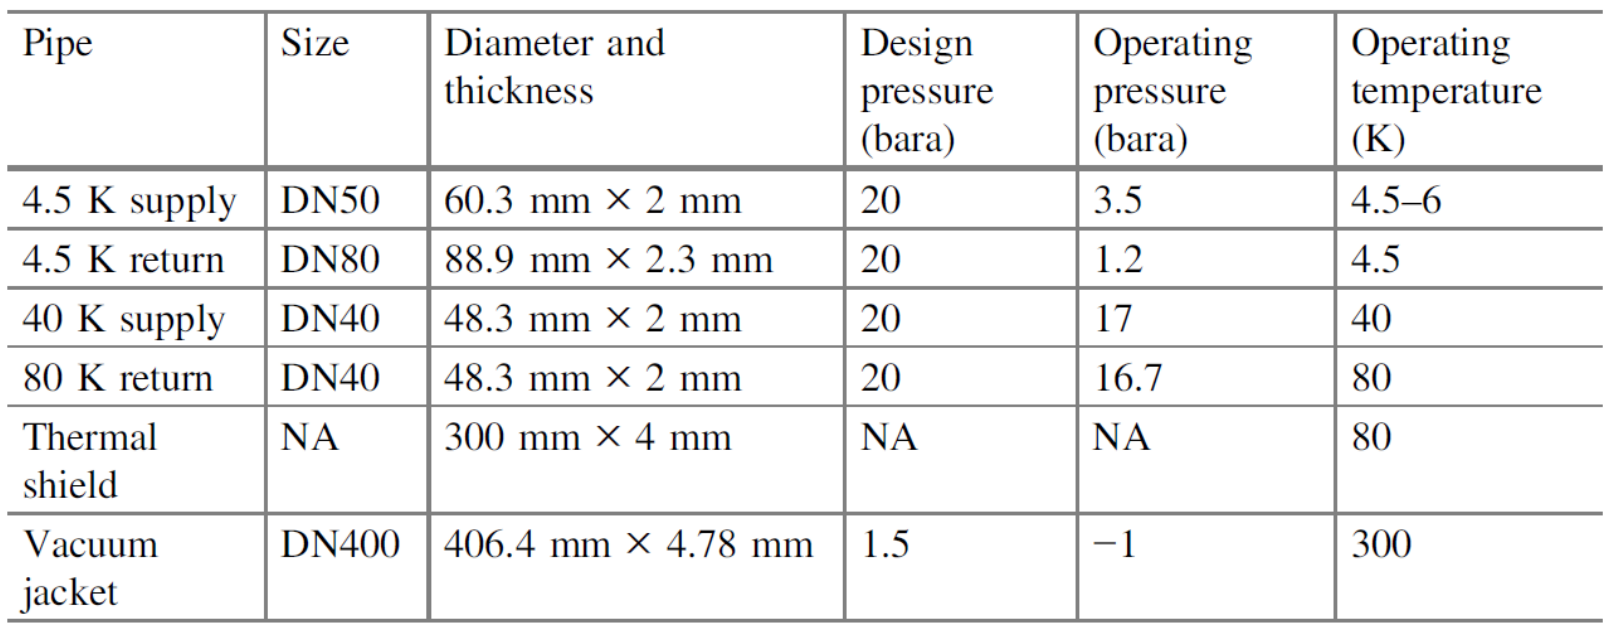
\includegraphics[width = \textwidth]{img/figure69.png}
    \caption{Sizes and operating conditions of the process lines, thermal shield and vacuum jacket.}
\end{table}
\subsubsection{SS304}
Type 304 stainless steel is a T 300 Series Stainless Steel austenitic. It has a minimum of 18\% chromium and 8\% nickel, combined with a maximum of 0.08\% carbon. It is defined as a Chromium-Nickel austenitic alloy. Grade 304 is the standard ``18/8'' stainless that you will probably see in your pans and cookery tools. These are some of its characteristics:
\begin{itemize}
    \item Forming and welding properties
    \item Corrosion / oxidation resistance thanks to chromium content
    \item Deep drawing quality
    \item Excellent toughness, even down to cryogenic temperatures, which are defined as very low temperatures
    \item Low temperature properties responding well to hardening by cold working
    \item Ease of cleaning, ease of fabrication, beauty of appearance
    \item Grade 304L is the low carbon version of 304. It does not require post-weld annealing and so is extensively using heavy gauge components (over about \SI{6}{\milli\meter})
    \item Grade 304H with its higher carbon content finds application at elevated temperatures
\end{itemize} 